\renewcommand\thetable{\arabic{chapter}-\arabic{table}}
%\renewcommand\thefigure{\arabic{chapter}-\arabic{figure}} 
\chapter{校舍資訊與耐震能力之關係模型}

在校舍耐震資料庫中,不同階段的調查資料有不同的校舍耐震能力指標,這些指標都是以數值形式來量化校舍建築物的耐震能力,有了此一數值後,可以快速找出有安全疑慮的校舍,根據耐震能力排序,甚至推算會需要多少預算來補強多少棟校舍等等,都可以使用此數值作為依據來達成,可以說是非常重要的校舍特性,然而要取得此一數值非常耗時耗力,如果有其他快速便宜的方法可以取得此一數值,那便可以大幅度的減少校舍耐震能力補強作業的所需要的時間與經費,因此本研究的第一個資料探勘目標,便是找出預測耐震能力索引的預測模型,得到此一預測模型後,便可以根據校舍的設計參數與現況作為輸入參數,快速的得到該校舍的耐震能力索引參考值。

初步評估階段資料的耐震能力指標是~$Is$~(seismic index)值,此一數值為專業人士於現場量測、調查後,使用國家地震中心的專家根據過往的實驗數據統計分析後,所設計出的一個評估表計算而得到的,為一初步的評估值,較詳細評估所計算的耐震能力指標可靠度來的低,但仍是校舍補強計畫初期的篩選工作中非常重要的數值。詳細評估和補強設計階段的耐震能力指標則是~$CDR$~值,~$CDR$~值是由專業人士根據校舍的設計與實際狀況建製結構模型,並進行非線性的推垮分析所得到的,此數值與建築物之設計參數為高度非線性的關係,也是最接近校舍建築物實際耐震能力的量化指標。

而除了數值量化的耐震能力指標外,本研究還將「校舍是否需要補強」($D\_isR$)這個二元指標作為耐震能力來作為校舍耐震資料庫中的第三個耐震能力指標,~$Is$、$CDR$、$D\_isR$~這三個耐震能力指標的預測模型,即為本研究所取得的第一個校舍耐震資料庫隱含知識,也是本研究所取得最直接相關於校舍設計參數與耐震能力之知識,以下便針對不同指標的預測模型的資料探勘流程與結果詳細介紹。

need modify

\section{是否需要補強與校舍設計之關係模型}

「校舍是否需要補強」此一指標其數值之基礎即為詳細評估的耐震能力指標~$CDR$~值,$CDR$~值超過~1~表示其耐震能力尚符合安全規範,反之,則是有安全疑慮,需要進一步補強或是拆除。而~$D\_isR$~則是標記各校設耐震能力是否足夠的二元指標,也是教育部的校舍耐震能力補強計畫中,前期篩選工作的最主要目標。找到這個指標與校舍設計、現況等參數的關係模型,與~$Is$~值和~$CDR$~值關係模型一樣,此一關係模型對於校舍耐震能力補強計畫中,初期的篩選工作可以有很大的助益,也可以輔助決策者編定預算、快速的根據狀況決定不同計畫年度補強的規模等。

本模型之構想為教育部或地方政府在訂定補強計畫或編列預算時, 常需有整體需補強校舍之數量統計,依照目前校舍耐震評估與補強之流 程如圖 1.1,需等到執行完詳細評估並通過審查決策後才能得之最後校舍 是否需補強或拆除,過程需耗大量時間與金錢。使用此預測模型,可於 短時間內,依據資料庫之現有資料,隨時立即做整體需補強校舍之預測。

\subsection{資料前處理}

本模型採用校舍資料庫中已存在之初步評估與詳細評估資料做為資 料探勘輸入參數,並以典型校舍、鋼筋混凝土建築、單邊走廊且廊外無 柱、無地下室、初步評估與詳細評估均顯示為已送出之資料做為此模型 資料選擇之條件篩選,模型資料經篩選過後,探勘模型中最重要的步驟 就是屬性欄位的挑選,本模型挑選之屬性集如圖 4.2,探勘模型之屬性挑 選分為輸入變數與輸出變數,本模型之輸出變數為校舍是否補強之欄位, 輸入變數則是我們用來預測輸出變數之所用變數,表 4.4 為本預測模型屬 性集內之屬性介紹與選擇說明。

\begin{multicols}{2}
\begin{itemize}
\item $S_{aD}$
\item 樓層數
\item 二樓樓地板長
\item 二樓樓地板深
\item 一樓樓地板面積
\item 教室柱總斷面積
\item 柱等效長度
\item 平面及立面對稱性
\item 軟弱層顯著性
\item 裂縫鏽蝕滲水等程度
\item 變形程度
\item 短柱嚴重性
\item 耐震性能 $E$ 值
\item 耐震指標 $Is$
\end{itemize}
\end{multicols}

\begin{description}
\item [一般工址或近斷層區域之工址設計水平譜加速度係數]
\cite{內政部營建署編輯委員會2005建築物耐震設計規範及解說} 即~$S_{aD}$ 一般工址或近斷層區域之工址設計水平譜
加速度係數,隨建築物基本振動週期 T 與工址短
週期與一秒週期之設計水平譜加速度係數𝑆𝐷 與𝑆𝐷 𝑆1
而改變,如表 4.5,𝑆𝐷與𝑆𝐷之值可由校舍所在位 𝑆1
置依規範查出。此係數是因校舍位址而改變,並 且其𝑆𝐷 與𝑆𝐷 為根據所在震區而訂定,藉由此係數
𝑆1
可間接知道該校舍可能靠近哪些震區,本研究採 用此一屬性,設想為可能某些地區的校舍可能其 接受補強之機率較高,因此嘗試將此屬性納入屬 性集。
\item [樓層數]
觀校舍資料庫之校舍樓層數,普遍落在 2 樓與 3 樓之間,並以 2 樓為最多數。再者校舍之樓層數 會影響到地震時之受力反應,與校舍之耐震能力 有某種程度上的關連,因此本研究將之納入本探 勘模型之屬性集。
\item [二樓樓地板長]
台灣中小學校舍中之典型校舍其建築形式較為固 定且普遍存有耐震能力較弱之現象,因此本研究 推測在這些典型校舍中應該存有某些特定尺寸之校舍其耐震能力較差,因此本研究將此屬性納入 屬性集做為本探勘模型之輸入屬性。
\item [二樓樓地板深]
台灣中小學校舍中之典型校舍普遍存有耐震能力 較弱之現象,本研究推測在這些典型校舍中應該 存有某些特定尺寸之校舍其耐震能力較差,因此 本研究將此屬性納入屬性集做為本探勘模型之輸 入屬性。
\item [一樓樓地板面積]
校舍之樓地板面積亦屬於建築形式之一環,因此 可視為該校舍之特有形式,本研究假設在典型校 舍中存有特定樓地板面積大小有其普遍對應之耐 震能力或某些尺寸之樓地板面積可能存有接受補 強較高的機率。
\item [教室柱總斷面積]
台灣中小學校舍其建築形式較為固定,教室柱之 多寡或其尺寸亦可視為建築形式中之一環,因此 本研究推測在這些校舍中,教室柱應該存有某些 特定總斷面積大小之校舍其耐震能力較差,因此 本研究將此屬性納入屬性集做為本探勘模型之輸 入屬性。
\item [柱等效長度]
  柱之等效強度~$T_{AC}$~其計算公式為:

  \begin{equation}T_{AC} = (4+1.8NF) \times ClaAc+(2.4+1.08NF) \times CorAc+2.6 \times InsAc\end{equation} 

  其中~$NF$~為樓層數,~$ClaAc$~為一樓教室柱總斷面積,~$CorAc$~為一樓走廊外柱總斷面積,~$InsAc$~為一樓隔間柱總斷面積,其公式為根據三種類結構柱之單位斷面積極限剪力牆度計算公式~\cite{su2008master}~之加總,本分析將此屬性加入探勘模型之最初原因為該公式內有教室柱、走廊外柱與隔間柱於一樓的總斷面積,而此一數值和,並且因補強施工其所補強之面積愈大其所花錢就愈多。本分析經建立多組模型與各種屬性集之測試均發現該屬性對模型之預測結果有一定影響。
\item [平面及立面對稱性]
[12] (國震中心,NCREE-03-049)初步評估表中參考 建築耐震設計規範之規定,若結構及其側向力抵 抗系統的平面幾何形狀具有凹角,超過凹角部分 於兩水平方向之結構尺寸同時大於沿該方向結構 總長之 15\%以上者,表示該結構具有凹角性,則 耐震能力折減為 0.95 倍;若該結構具有凹角,但 超過凹角部分於任一方向之結構尺寸不足沿該方 向結構總長之 15\%,且無其他平面及立面不規則 之情況,則耐震能力不予折減;若該結構不具任 何凹角,且無其他平面及立面不規則之情況,則 耐震能力增加為 1.05 倍。根據上述可知該屬性為 影響校舍耐震能力之屬性之一,校舍是否補強其 最相關的為評估完之耐震能力,因此本研究將該 欄位加入屬性集。
\item [軟弱層顯著性]
[12] (國震中心,NCREE-03-049)若結構物之一樓因 為使用性等考量,而使得二樓以上 RC 牆或磚牆於 一樓中斷,致使一樓之極限層剪力強度與勁度降 低,將造成地震力作用時變形集中,以致於韌性 用盡,建築物就發生軟弱層破壞。故本表格依據 牆體中斷的程度折減其對應之耐震能力,若 2/3 以上牆體中斷,則耐震能力折減為 0.8 倍;若 1/3 至 2/3 之牆體中斷,則耐震能力折減為 0.9 倍;若 1/3 以下之牆體中斷,則不折減其耐震能力。依此敘 述得知軟弱層顯著性會影響結構物之耐震能力, 結構物之耐震能力愈低,其接受補強的機率就愈 高,因此本研究將此屬性納入本屬性集。
\item [裂縫鏽蝕滲水等程度]
[12] (國震中心,NCREE-03-049)鋼筋混凝土構材若 具有裂縫,代表混凝土品質不良或強度不足;保 護層不足等因素使得鋼筋銹蝕膨脹,鋼筋銹蝕將 會降低構材之強度,鋼筋銹蝕膨脹亦會導致混凝 土剝落,並加速鋼筋鏽蝕的程度,這些因素都會 影響結構物的耐震安全,故以結構物整體之裂縫 銹蝕滲水等程度作為調整項目。若稍有裂縫銹蝕 滲水等情形,則耐震能力折減為 0.95;若裂縫銹 蝕滲水等情形較為嚴重,則耐震能力折減為 0.9; 若無,則不折減其耐震能力。根據上述可知該屬 性為影響校舍耐震能力之屬性之一,校舍是否補 強其最相關的為評估完之耐震能力,因此本研究 將該欄位加入屬性集。
\item [變形程度]
0.9 倍;若無,則不折減其耐震能力。依上之敘述 可知該屬性為初步評估表中結果之影響因子,可 影響評估最後結果之耐震能力,耐震能力愈低其 接受補強機率就愈高,因此將之加入本屬性集。
\item [短柱嚴重性]
[12]一般老舊校舍之柱箍筋間距多為 20cm 至 30cm 左右,其剪力強度不高,且老舊校舍於設計時假 設為純梁柱系統,並沒有考慮教室窗台及樓梯廁 所等牆壁開氣窗所造成之短柱效應,然而這種短 柱效應將會使得剪力容量不足之柱於地震時發生 非預期之剪力破壞,導致結構韌性不足,若該校 舍有過多之柱受到短柱效應之影響,將易造成校 舍瞬間倒塌。故若校舍因窗台或氣窗造成短柱現 象之柱根數達到全部柱根數之 50\%以上,則耐震 能力折減為 0.9 倍,若不足 50\%則不予折減其耐震 能力。值得注意的是,短柱嚴重性具有方向性, 故評估時只需考慮評估方向之短柱比率是否超過 一半即可,另一方向開窗等因素造成之短柱效應 不需考慮。短柱效應其影響校舍之耐震能力相較 於其他影響因子相對於較大,校舍評估出來之耐 震能力幾乎是校舍是否需補強之主要因素,因此 該欄位更應該加入本探勘模型之屬性集。
\item [耐震性能 $E$ 值]
耐震性能 E 值為初步評估中之初步計算耐震性 能 , 其 計 算 公 式 為 「 0.354*NF*(TAc+TAw)/((-1+6*NF)*(0.4*SaD)*Af)」,從其公式可得知,初 步評估法中,亦將 NF 樓層數、TAc 柱等效強度與 SaD 列入計算式中,Af 為總樓地板面積、Taw 為牆 總斷面積。本模型之預測目標為校舍是否需補 強,因此將該屬性列入本屬性集。
\item [耐震指標 $Is$]
耐震指標 Is 為初步評估最後之評估值,[12]以 80 分作為耐震能力堪慮之標準,若校舍調查所得之 耐震指標 Is 值低於 80 分,表示其耐震能力頗為不 足,確有耐震疑慮,若有相當於 475 年回歸週期 之地震發生時,將有嚴重損壞或倒塌之疑慮,應 最優先進行耐震能力之補強設計與施工;耐震指 標 Is 值介於 80 分及 100 分,表示校舍耐震性之安 全係數尚不符合耐震設計規範對於此等重要性建 築物之耐震需求,仍有耐震性能不足之疑慮,若 有相當於 475 年回歸週期之地震發生時,將有可 能發生嚴重結構上之破壞,其耐震能力之提升(補 強工程)列為次優先對象;耐震指標 Is 值高於 100 分,表示其尚無耐震疑慮,若有相當於 475 年回 歸週期之地震發生時,應不至於發生嚴重結構上 之破壞。雖然根據上述耐震指標 Is 低於 100 分就 須接受耐震補強,但根據觀察校舍資料內資料, 初步評估結果 90 至 100 分進行詳細評估後,絕大 部分都不須進行補強,80 分以下 70 分以上也有一 些進行詳細評估後也是裁定不需補強,因此雖然耐震指標 Is 不是最後決定補強之最後依據,但也 具有一定之影響性。本研究最後決定將此屬性加 入本屬性集。
\end{description}

\subsection{資料探勘}

探勘模型於建立屬性集後,接著即是依挑選之屬性設定最適合該探
勘方法之資料格式及資料類型。本模型之參數設定如表 4.6。

本研究原先採用支援向量機與 CHAID 進行資料探勘之建模,選擇此 二種探勘方法,主因為本研究之預測目標,是否需補強其資料類型為 「名義」,名義之資料類型其一般採用之探勘方法為支援向量機與 CHAID,CHAID 經初步測試本研究之預測目標,其效果不錯,但支援向 量機其結果不如預期的好,因此本研究後來轉向使用類神經網路與 CHAID 探勘方法,使用前處理完之 2153 筆資料並挑選屬性集內之欄位, 將整體資料分為訓練區 70\%與測試區 30\%,做為探勘模型之訓練方法。 最後再挑一組結果較好之模型保留並以另外挑選之獨立 50 筆校舍資料進 行結果測試,測試結果敘述於第五章。本模型之訓練結果如表 4.7,表中 之正確率為預測值與校舍資料庫值之比較。


\begin{table}[hbtp]
  \begin{center}
    \caption{Result of the D\_isR}
    \label{tab:d_is_r_result}
    \large
    \begin{tabular}{l c c c c}
      \hline
       & \multicolumn{2}{c}{ANNs} & \multicolumn{2}{c}{CHAID} \\
       & Training & Testing & Training & Testing \\
      \hline
     正確率 & 93.03\% & 91.41\% & 91.14\% & 88.59\% \\
      \hline
      \end{tabular}
  \end{center}
\end{table}

\subsection{結果}

















\section{Is 值與校舍設計之關係模型}

校舍耐震資料庫中的初步評估資料表的耐震能力索引是為~$Is$~值,初步評估是校舍耐震能力補強作業中,很重要的篩選過程,因為建築物的詳細評估所需要的金額極高,評估需要的時間也很長久,因此需要一個速度、價錢和可靠度都可以接受的評估方法,用比較短的時間找出耐震能力有疑慮的校舍,盡早處理。而地震中心所設計的初步評估表即為一個速度、價錢和可靠度都可以接受的評估方法,只要根據建築物的設計參數,像是樓層數、長度、深度、柱子尺寸以及校舍現況等,就可以快速的得到一個極具參考價值的耐震能力指標,而其計算的原理也與詳細評估的耐震能力指標索引~$CDR$~值一樣,為耐震容量與耐震需求的比。找出~$Is$~值與校舍設計參數之間的關係模型,可以進一步分析初步評估表中各種數據的重要性,並將結果回饋到此一初步評估表,將初步評估表調整的更為精簡,負責評估的人員也可以更快速的完成此意評估表格。

% The proposed prediction model, based on data-mining technology, has six steps – business understanding, data understanding, data preparation, modeling, evaluation, and deployment – as recommended in the cross industry standard process for data mining (CRISP-DM) proposed by Chapman et al. (2000) (Fig. 9). The objective of this work is to construct a prediction model for the aseismic ability indices of school buildings and collect complete data. Hence, the major tasks are data preparation, modeling, and evaluation. Fig. 10 shows the procedural plan based on needs and the methods chosen. 

\subsection{資料前處理}

首先,從國震中心的校舍耐震資料庫中,將各棟校舍的~$Is$~值與其校舍的相關資料挑出並整合在一起,第一步是過濾掉明顯不合理的錯誤資料,這些資料通常是人為的錯誤造成的,而過濾的方法則是使用國陣中心建議的過濾條件:

\begin{itemize}
\item 校舍總長或總深度超過兩百公尺
\item 有任意牆厚度超過五十公分
\item 有任意柱的長或寬超過一百公分
\item 柱間垮距超過八公尺或小於兩公尺
\end{itemize}

大約有八百筆資料符合這組基本的過濾條件,而在初步的過濾之後,前處理的第二個步驟則是減少資料屬性的維度,主成分分析(principal component analysis)是很常使用的資料前處理方法,這個分析方法可以找出所有資料屬性中,重要度較高的屬性,它是把原始的多個資料屬性,透過向量轉換的方式,線性組合出主要的資料屬性。

% Roughly 800 bits of valid data are obtained. After filtering using these conditions. Principal component analysis (PCA) is then used to reduce the dimensionality of data attributes. Notably, PCA, a very common data preparation method, can identify very important attributes among various attributes. The goal is to convert the original variables through vector transition into mutually independent variables of a linear combination. The ideal situation is that principal components obtained from linear combination retain most of the information of original variables.

校舍的分群則是基於校舍的設計模式,目標是要找出校舍建築物的幾種特定設計模式,也就是要分析校舍的幾何設計參數、柱量、牆量等等,經過不斷的測試及調整,最後找出了五個主要成分屬性:

\begin{itemize}
\item 走廊柱資訊
\item 教室柱資訊
\item 強設計資訊
\item 牆量資訊
\item 柱量資訊
\end{itemize}

% Clustering analysis of school buildings is based on the design patterns of school buildings; the goal is to find several design patterns. Hence, the attributes for analysis are the geometric information of school buildings, such as dimensions and quantity of walls and columns, and width and height of school buildings. Other attributes, such as year of construction and locale, may not be incorporated into PCA analysis. After continuous testing and adjustment, five major attributes are obtained and the importance of constitutional fields is considered as the basis for naming. The five attributes are as follows: corridor column information; classroom column design information; wall design information; data for number of walls; and, data for number of classroom columns.

在前面的處理完成後,還使用分群分析將校舍分群,以幫助後續的~$Is$~值關係模型的建立,分群的目標是將校舍依照不同的設計模式特性區分開來,將相近設計的校舍放在同一群集,分群的依據是主成分分析法所找出的五種主要校舍設計相關屬性,圖~\ref{fig:spss-cluster}~是使用~SPSS Clemitine~進行此一分群分析時的節點設計圖,分別使用的~K-means~和~Two-Step~兩種分群演算法,其參數設定如下:

\begin{figure}[hbtp]
  \begin{center}
    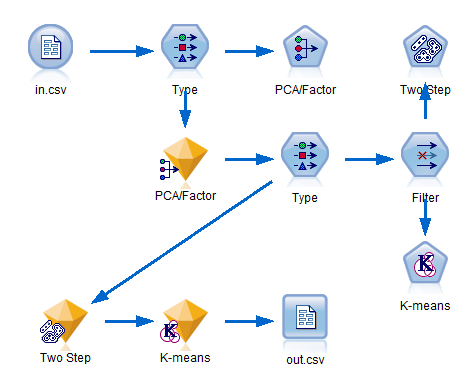
\includegraphics[width=0.7\textwidth]{figures/spss-cluster.png}
    \caption{Node configuration in clustering by SPSS clementine} 
    \label{fig:spss-cluster}
  \end{center}
\end{figure}

% After data preparation, clustering analysis is utilized to find hidden design patterns of school buildings. This study uses the K-means and two-step clustering methods. Fig. 11 shows the node deployment for clustering using the SPSS Clementine (2007) software. The parameter choices for the two methods are as follows.

\subsubsection{K-means}

此一分群方法最重要的設定參數是初始的群集數~$k$~,雖然有許多研究都在研究如何找出最佳的~$k$~值,但是目前仍沒有一個方法可以宣稱它找到~$k$~值是最佳的,唯有對該領域的專業了解以及詳細的測試才能得到最佳的 $k$ 值,在本分析案例中,~K-means~分群的停止條件是設定為~20~次迭代,如果~$k$~太大,那會造成分群結果無法在~20~次迭代內收斂,如果~$k$~小於~6~,則分群的結果就可以在~20~次迭代內完整的收斂,每筆資料都會故底定在所屬的群集內,不在變動,最後挑選的~$k$~值是~5~,而根據此意參數的分群結果可以找出三個主要的校舍群集,分別的比例是~28\%~、~56\%~和~16\%~。

% The most important parameter with this clustering method is the initial group, k. Although many researchers have developed methods for choosing the initial K value, no method can confirm that it has found the best K value. The best K can be found only based on researcher understanding and problem testing. In this study, K-means clustering is set to stop after 20 iterations. If the K value is too large and cannot be completely converged after 20 operations, some data points will continue to change the clusters to which they belong. When the K value is reduced to <6, Clustering models can be completely converged after 20 iterations, become stable, and no longer change cluster label of all data bit. The K value chosen is 5, and three major clusters are obtained. The remaining two clusters have few data and are considered outliers. The distribution of three major clusters are 28\%, 56\%, and 16\%.

\subsubsection{Two-Step}

Two-Step~分群有兩個優點,一是複雜度不高,運算時間與資料數量間之關係為線性關係,第二個優點就是不需要由人工決定分群的群數,演算法即可自己根據資料狀況決定,操作人員只需給予上下限,在本分析中,上下限的設定為最少兩個群集,最多八個群集,而最後的分析結果是所有的資料都被分到兩個群集中,分別佔了~54\%~和~45\%~。

% This clustering method has two features. The first is enhanced scalability. The algorithm has low complexity. Computing time does not grow nonlinearly as data volume increases. The other feature is that it can determine the number of clusters, unlike K-means clustering, which requires manual designation of parameters. However, this work can designate the upper and lower limits for the number of clusters. This work sets the limit to 2–8 clusters based on experience with K-means clustering. Consequently, all data are divided into two clusters, accounting for 54\% and 45\% of all data.

此資料探勘分析還用了十群交叉驗證來驗證結果的可靠度,因此資料前處理的最後一個步驟就是將整理好的資料隨機分為十組。

% This work uses 10-fold cross validation to validate the prediction model. After preparation, data are grouped by first dividing data randomly and equally into 10 clusters. One cluster is then chosen as a dataset for validation and the remaining nine clusters are combined into one training dataset.

\subsection{資料探勘}

完成資料前處理,將校舍的群集分好之後,才開始建立~$Is$~值與校舍設計參數的關係模型,本分析使用了廣義線性模型、線性回歸和類神經網路三種分析方法,每種方法都有三種分析資料群,分別為先經過~K-means~分群的資料、先經過~Two-step~分群的資料及沒有先經過分群的資料。圖~\ref{fig:spss-mining}~為使用~SPSS Clemitine~分析時的節點設計圖。以下分別對三種分析方法的參數設定作說明。

\begin{figure}[hbtp]
  \begin{center}
    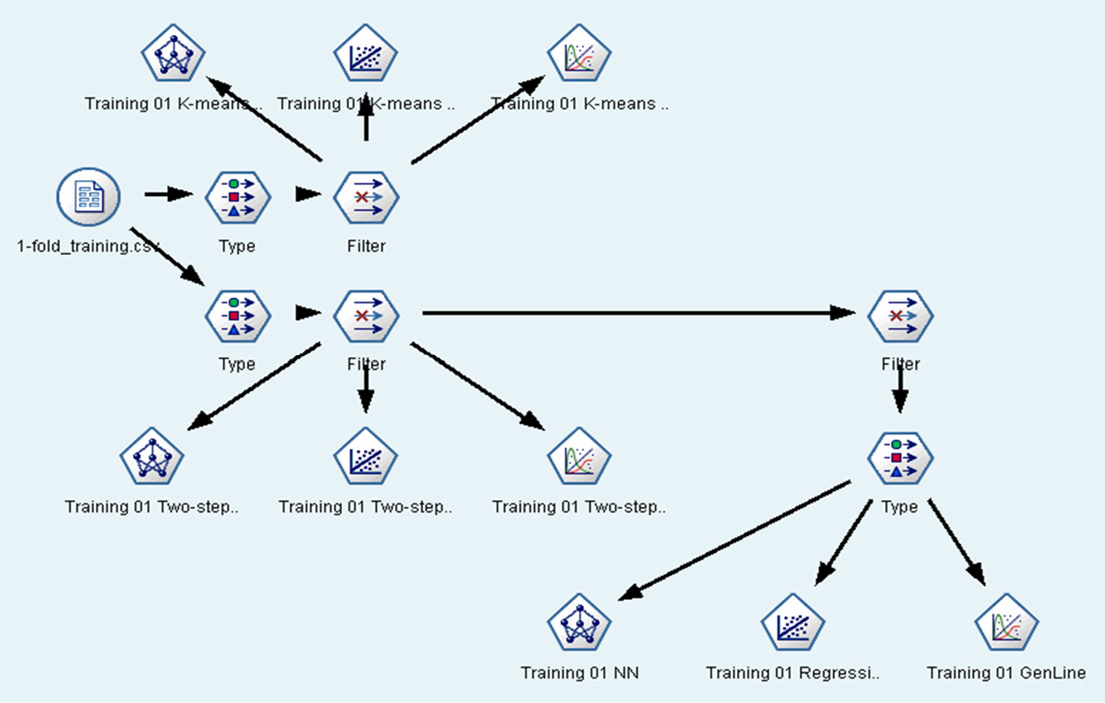
\includegraphics[width=1.0\textwidth]{figures/spss-mining.png}
    \caption{Node configuration built by SPSS prediction model} 
    \label{fig:spss-mining}
  \end{center}
\end{figure}

% The prediction model is built only after clustering is completed. This work uses a GLM, simple regression, and ANNs to build the prediction model based on three groups of data – not clustered in advance, clustered by K-means, and clustered by the two-step method in advance. In total, nine prediction models are generated. Fig. 12 shows the node configuration within SPSS Clementine. Below are the parameters chosen for the three methods. 

\subsubsection{廣義線性模型}

廣義線性模型(GLM)是假設在輸入參數和預測目邊之間有一個可以用連結函數表達的關係,這個連結函數可能是指數函數、對數函數、Logistic~函數等,經由一些測試資料的測試,我們選擇使用對數函數作為連結函數,並且根據實際的資料分佈選擇了常態分布作為輸入參數的分佈函數,而關係模型的分布也選擇常態分佈,因其表現較其他分布形式較好。

% The GLM assumes a relationship between input variables and a predictor; this relationship can be built by a link function such as identity function, log function, logit function, or power function. After available link functions testing on some data, the prediction model performs best when using log function as the link function; hence, this work chose the log function. The distribution function of the predictor is based on the actual distribution of data. This work chose the normal distribution, which is close to the real data distribution. The prediction model constructed using the normal distribution performed better than those with other distribution types.

\subsubsection{Simple Regression}

線性回歸是選擇使用最小平方根法來建立校舍建築物的設計參數與其耐震能力~$Is$~之間的關係,這也是最常使用的回歸方法之一。

% Simple regression in this work uses the least square method by adopting the building design parameters as independent variables $X$ and the aseismic ability of buildings as dependant variables $Y$. The linear equation between regressed design parameters and aseismic indices serve as the model for predicting aseismic ability $Y$ based on building design parameters $X$.

\subsubsection{Artificial Neural Networks}

類神經網路需要決定的參數包括隱藏層的數量、每層的神經元數量、學習率、停止條件等,除了直接設定神經網路的參數,還有一些方法可以使用,例如 dynamic、multiple 或是~prune method~可以用來調整並找出最佳的神經網路大小和結構,dynamic method 是從一個小型的神經網路開始(兩個隱藏層、每層兩個神經元),慢慢成長,並且比較成長前後的神經網路效能與結果,~multiple method~ 則是同時產生各種不同的神經網路,並且一起訓練到達停止條件,然後在從中挑選出表現最好的一個,而~prune method~則是從一個大的類神經網路開始,慢慢的把重要度低的神經元節點拿掉。本分析最後挑選的是~exhaustive prune method~,是~prune method~的一種修改形式,對於節點的篩選要求較高,是所有方法中最花時間的,但是通常也可以找到最好的結果。其他的類神經網路設定參數為:初始的神經網路為兩層隱藏層,其中一層有~30~個神經元、一層有~20~個神經元,停止條件為~250~個訓練循環,在這個設定下,~exhaustive prune method~是表現最好的方法。

% Generally, ANNs must decide on such parameters as number of hidden layers, number of neurons in each layer, learning rate, and stop condition. Aside from directly setting these parameters, methods such as dynamic, multiple, and Prune methods are available for adjusting and finding the optimal size and structure of the neural network. The dynamic method starts with a small neural network (two hidden layers with two neurons for each layer), expands network size gradually, and decides on the further expansion based on model performance before and after expansion. The multiple methods constructs multiple neural networks simultaneously, trains all neural networks to reach the ``stop condition,'' and then selects the group with the best performance. In contrast with the dynamic method, which slowly builds a large neural network from a small one, the Prune method first builds a large network and then removes neurons with low importance based on training. This work chooses the exhaustive Prune method, a special application of the Prune method. The initial neural network has two hidden layers, one with 30 neurons and the other with 20 neurons. The stop condition is set to 250 training cycles. Under this limit, the prediction model built by the exhaustive Prune method performs best.


\subsection{驗證}

驗證有兩個主要的目的,一是確保資料探勘找到的關係模型的可靠度,而不會找到只適用於該組訓練資料集的關係模型,第二個目的是可以用來作為比較不同分析方法的指標數據,本分析使用的驗證方式是十群交叉驗證,這個方法將所有的資料等分成十份,每次挑選九組出來作為訓練資料集,留下一組作為驗證資料集,如此可以得到十組模型以及其可靠度的指標,求此十組指標平均值即可得到代表此關係模型的可靠度代表值,而本分析所選擇的指標有三個,線性關係、絕對平均誤差(Mean Absolute Prediction Error, MAPE)以及命中率。

% Validation work has two purposes. The first is to ensure model reliability instead of to generate only good performance during data training. The second is to serve as a benchmark for comparing the performance of different prediction models. This work uses 10-fold cross validation to assess and compare the performance of prediction models. This method divides a fixed amount of data into 10 groups, conducts 10 rounds of model building and validation, chooses a different group of data for testing, trains the model with remaining nine groups of data, and uses test group data to validate model accuracy. After validation for 10 times, the accuracy of the 10 models is obtained and their average is taken as the accuracy of this algorithm. This study uses linear correlation, mean absolute prediction error (MAPE), and hit rate as the indices for comparing the prediction model performance.

\subsection{結果}

此資料探勘分析會產生九個校舍耐震能力與校舍建築設計資訊間的關係模型,包括直接使用~GLM~、線性回歸和類神經網路的三組,混合使用~K-means~或是~Two-Step~分群的六組,要比較其優劣我們使用了線性關係~$R$~、~MAPE~和~hit rate~三個指標,其中線性關係越高表示兩者之間越接近,也代表著關係模型的正確性,而~MAPE~ 的是用來表示關係模型誤差之數值,由於關係模型不可能完全沒有誤差,即使有非常高的線性關係也是會有誤差,因此會使用~MAPE~作為判斷其誤差程度的參考。

%並配合十群交叉驗證,其中線性關係 $R^2$ 之公式為:

% This work constructed nine prediction models; three are directly generated by the GLM, simple regression, and ANNs. The mixed model of K-means and two-step clustering generated three prediction models. Hence, nine models were obtained and 10-fold cross validation is used to compare the performance of the three reference indices – R2, MAPE, and hit rate. Notably, R2, the linear correlation is

%\begin{equation} R = \dfrac{\sum{(\hat{y_i} - \tilde{y})^2}}{\sum{(y_i - \tilde{y})^2}} \label{eq:RSQ}\end{equation} 

%其中 $y_i$ 是校舍的實際耐震能力指標 $Is$ 值, $\hat{y_i}$ 則是透過此關係模型的到的推估耐震能力指標值,$\tilde{y}$ 則是所有資料的 $Is$ 值之平均,透過此一公式即可得到實際的 $Is$ 值與透過關係模型得到的推估值之間的線性關係,線性關係越高表示兩者之間越接近,也代表著關係模型的正確性。MAPE 的公式為:

% where yi is the aseismic CDR of school buildings obtained using nonlinear analysis of the database, yi is the CDR obtained from the prediction model, and y~ is the average aseismic CDR of school 651 buildings obtained using nonlinear analysis. The correlation between aseismic CDR of school buildings obtained via the prediction model and nonlinear analysis can be determined based on linear correlation. A high CDR indicates a strong correlation and many opportunities to make correct predictions. The MAPE is derived as

%\begin{equation} MAPE = \dfrac{\sum{\dfrac{y_i - \hat{y_i}}{y_i}}}{N} \label{eq:MAPE}\end{equation} 

%其中 $N$ 是資料總數,MAPE 的是用來表示關係模型誤差之數值,由於關係模型不可能完全沒有誤差,即使有非常高的線性關係也是會有誤差,因此會使用 MAPE 作為判斷其誤差程度的參考。
% where N is the number of samples. The MAPE is used to judge the  degree of error of prediction models as the prediction result always has errors, although the prediction mode has an adequately high R2. The hit rate is derived as hit rate

%\begin{equation} hit\ rate = \dfrac{ \sum{I\{(1 - \alpha)y_i \le \hat{y_i} \le (1 + \alpha)y_i \}} }{N} \label{eq:hitrate}\end{equation} 

%其中~$0 \le \alpha \le 1$~,且~$I\{L\} = 1$~。hit rate~是用來判斷關係模型的正確率的。
在本分析中,我們設定了兩個~$\alpha$~值作為計算命中率(hit rate)指標用,分別是~0.1~和~0.2~,表~\ref{tab:is_result}~列出了這九個關係模型使用這三個指標配合十群交叉驗證所得到的數值,表現最好的關係模型是先使用~K-means~分群再使用~GLM~所建立的,第二好的則是先使用~Two-step~分群再使用~GLM~所建立的,圖~13~是先使用~K-means~分群再使用~GLM~所建立模型的實際~$Is$~值與使用模型得到的~$\hat{Is}$~值的比較圖,資料點的回歸取現的斜率非常接近~1~,可以看得出來兩者之間的相關度非常高。如果單看模型的線性關係表現,類神經網路的表現比~GLM~ 和線性回歸都要來的好,這也可以驗證校舍的耐震能力與其設計參數之機善一個非線性的關係,而雖然~GLM~整體的排名較~ANN~來的好,但是~hit rate~卻是~ANN~表現的比較好,但是看到~MAPE~又會發現~ANN~的~MAPE~較大,因此我們建議在~$Is$~值的關係模型的挑選,可以依據應用的需求來決定,如果需要較高準確率的時候,建議使用~ANN~,如果是需要降低整體的誤差,則建議使用~GLM~。如果先使用分群方法將校舍資料根據設計參數分出不同群集後,再對不同群集分別探勘其耐震能力與設計參數的關係模型,結果會比沒有先分群要來的好一些,探討其原因,是因為典型校舍已經是校舍建築物的一個子集合,而此子集合的特性已經非常接近,因此再進行分群也不會有顯著的改善。


\begin{table}[hbtp]
  \begin{center}
    \caption{Cross-validation result of the prediction model}
    \label{tab:is_result}
    \scriptsize
    \begin{tabular}{l c c c c c c c c c}
      \hline
       & K-means & Two-step & ANNs & K-means    & Two-step   & Regression & K-means & Two-Step & GLM \\
       &   ANNs  &   ANNs   &      & Regression & Regression &            &   GLM   &   GLM    & \\ 
      \hline
   	   R              & 80.21\% & 81.78\% & 80.76\% & 72.16\% & 72.16\% & 72.15\% & 87.41\% & 87.11\% & 87.05\% \\
       MAPE           & 28.69\% & 26.64\% & 26.51\% & 46.06\% & 46.05\% & 46.05\% & 24.68\% & 24.70\% & 24.71\% \\
       hit\_rate(0.2) & 53.12\% & 54.29\% & 54.31\% & 40.16\% & 40.17\% & 40.21\% & 48.82\% & 48.64\% & 48.52\% \\
       hit\_rate(0.1) & 27.71\% & 28.72\% & 28.75\% & 21.13\% & 20.98\% & 21.09\% & 25.05\% & 25.16\% & 25.16\% \\
      \hline
       Rank & 6 & 4 & 3 & 9 & 7 & 8 & 1 & 2 & 4 \\
      \hline
      \end{tabular}
  \end{center}
\end{table}

% When 0<a<1 and I{L} = 1, hit rate is utilized to determine the percentage of data predicted correctly by the prediction model, that is, prediction model accuracy. In this work, the hit rate is ranked by setting a equal to 0.1 and 0.2, which are utilized as two assessment indices that average and rank the performance of accuracy. Table 1 lists the assessment indices of the nine prediction models. The prediction model that performs best is that built using the GLM with K-means clustering. The second best prediction model is that built via the GLM with two-step clustering. Fig. 13 compares the actual CDR and CDR obtained using the K-means and GLM prediction models. The slope of the regression curve equation approaches 1, indicating a strong correlation between school building design data and aseismic ability of building. However, the scattered distribution of actual data points corresponds to a high R2 and high MAPE. After a thorough comparison of the nonlinear analysis by ANNs, the GLM, and linear analysis by simple regression, the ANNs perform better than the GLM and linear analysis by simple regression all aspects, confirming that the design parameters of school buildings have a nonlinear relationship with aseismic ability, which conforms to the fact that the aseismic CDR in this work is obtained using nonlinear analysis. Although the GLM ranks high in comprehensive assessment, its hitate is worse than that of ANNs; ANNs also have a higher MAPE. Hence, it is possible to determine which prediction method is suitable based on actual needs when predicting the aseismic ability of school buildings. We recommend using ANNs for accurate prediction of the aseismic abilities of school buildings; however, the drawback in using ANNs is that the prediction model generated is a black box. We recommend using the GLM to minimize total error. When building prediction models by clustering first and then comparing the performance of the three assessment methods, the prediction model built with clustered data performs slightly better than those built directly, indicating that traditional school buildings are already a subcluster of various architectural patterns. One feature of subclusters is their weak correlation with the aseismic ability of school buildings. Hence, information added to the cluster will not markedly improve prediction model quality.

由於校舍補強預算和時間有限,因此其執行的優先順序就會依照評估得到的耐震能力作為參考排序,因此本分析還用此實際的應用作為另一個評量關係模型優劣的指標,此指標將所有的校舍依照其~$Is$~值排序後,照順序等分成~10~群,另外在用關係模型得到的~$\hat{Is}$~排序,一樣照順序等分為 10 群,接著比較每筆校舍所分配到的群集,如果實際所屬的群集編號和關係模型得到的群集編號一樣,則誤差(error)為~0,如果差了一號,則誤差為~1,差了兩號則誤差為~2,表~\ref{tab:is_seq_result}~即為九組關係模型的排序誤差結果。可以發現表現最好的一組仍然為先使用~K-means~分群再用~GLM~ 探勘所得到的關係模型,其誤差小於~1~的資料比例為~70.8\%,誤差小於~2~的資料比例則有~88.9\%~。

% The budgets and priorities for reinforcing school buildings are based on the aseismic abilities of school buildings. This work analyzed the sequencing result of aseismic ability of school buildings by sequencing school buildings based on CDR values, dividing them into 10 equal zones, and comparing the zone number of actual and predicted values. Table 2 shows the zoning result. When Error = 0, the predicted and actual values have the same zone number; when Error = 1, predicted and actual values are in adjacent zones; when Error = 2, predicted and actual values are separated by one zone. The prediction model built by the GLM with K-means clustering performs best. The zoning error of this prediction model <1 is 70.8\%, and the zoning error <2 is 88.9\%, indicating that the prediction model already has sufficient accuracy when sequencing is used.

\begin{table}[hbtp]
  \begin{center}
    \caption{Sequencing analysis of prediction of aseismic ability}
    \label{tab:is_seq_result}
    \scriptsize
    \begin{tabular}{l c c c c c c c c c}
      \hline
       Error & K-means & Two-step & ANNs & K-means    & Two-step   & Regression & K-means & Two-Step & GLM \\
             &   ANNs  &   ANNs   &      & Regression & Regression &            &   GLM   &   GLM    & \\ 
      \hline
	   0  & 32.8\% & 35.0\% & 33.9\% & 33.4\% & 34.1\% & 33.3\% & 35.6\% & 34.9\% & 35.0\% \\
	   1  & 36.0\% & 35.2\% & 36.5\% & 35.4\% & 34.2\% & 35.5\% & 35.2\% & 35.9\% & 35.7\% \\
	   2  & 17.5\% & 15.2\% & 16.2\% & 16.6\% & 17.1\% & 16.4\% & 18.1\% & 17.3\% & 17.5\% \\
	   >2 & 13.7\% & 14.6\% & 13.5\% & 14.6\% & 14.7\% & 14.8\% & 11.1\% & 11.9\% & 11.8\% \\
      \hline
      Rank & 5 & 5 & 4 & 7 & 9 & 8 & 1 & 2 & 2 \\
      \hline
      \end{tabular}
  \end{center}
\end{table}


















\section{CDR 值與校舍設計之關係模型}

校舍耐震資料庫中,詳細評估表的耐震能力索引~$CDR$~值是用來評估校舍是否需要補強、甚至是拆除的最重要依據,此數值需要由專業人士進行完整且詳細的評估,此數值的取得非常耗時耗力,且評估需要之經費也不便宜,,是一個與校舍結構材料、設計與現況等參數之間為高度非線性的關係的數值,如果能夠取的此一關係模型,對於校舍耐震能力補強計畫來說,絕對可以有很大的幫助。

\subsection{資料前處理}

人工輸入的資料很容易發生單位錯誤或是格式不正確的資料,而資料的品質對於資料探勘的結果優劣影響很大,因此需要在資料前處理時把這些問題都處理過,資料前處理的最主要目標是讓處理過的資料能夠很確實的反映出分析問題所要尋找的資料特性,使用的方法包括資料過濾、屬性過濾、新屬性的生成等,首先,本分析中第一個前處理工作就是資料過濾,要把有問題的資料,不合理的資料都過濾掉,過濾的條件則是依照國震中心所建議的典型校舍特性的過濾條件:

% Manually inputting data may result in incorrect units or formats because controlling data quality in the real world is difficult. Hence, it is necessary to pre-process data before building the relational model. Quality, as an important part of soft computing and data analysis, has considerable influence on subsequent analytic results or even on the reliability of the generated model. Apart from the actual data, the researcher also refers to expert advice from NCREE for data pre-processing. The main target of data pre-processing is to ensure the accuracy and adjustment of the data in a format that clearly reflects the target of analysis. Pre-processing includes data screening, property screening, and new property synthesis. Data screening is divided into two stages. The first stage is the rationality screening of the data. Pre-existing mistakes are unavoidable because the data in the School Building Database were entered manually; the obligation is to identify such mistakes. Most of the school buildings were I-type shaped buildings; a very common design. . With regard to the properties of these school buildings, the NCREE (2005) suggests the following screening conditions:

\begin{itemize}
\item 校舍深度介於六到二十公尺之間
\item 校舍垮距介於二到八公尺之間
\item 每間教室至少有一個垮、兩個柱
\item 是否有短住效應 % The number of columns in the classroom is low
\item 校舍的破壞地表加速度是長向較小
\end{itemize}


由於並不是所有的校舍都有進行過詳細評估,因此第二個步驟就是要挑選出同時有基本設計資料以及詳細評估的~$CDR$~值的資料,接著,由於校舍資料庫中的原始資料,每棟校舍都有上百個資料屬性,因此接著要對屬性進行篩選與合併,與國震中心之專家討論過後,挑選過濾掉大部分的屬性,但是仍然有約三十多個屬性,因此為了能夠繼續減少資料屬性,本分析接著還繼續對這些資料的屬性進行分類,根據其屬性分布挑選出一組典型校舍子集來分析,這個挑選出來的子集其特性為:

% In the second stage, choosing school buildings with both basic design parameters and minimum destruction ground acceleration is necessary because not all school buildings have detailed information.According to the raw data in the seismicassessment database for school buildings, each data set contains hundreds of properties. Based on our judgment with expert which are non-structural and low importance, and synthesize some properties with similarity. There are still more than 30 properties left after this reduction process. This study further classifies school building records into subsets based on similarities in property values, and chooses one subset with major population as the data set for further studying. After the classification of school buildings, we try to do further reduction and finally determine a set of key properties which is optimal to represent the seismic characteristics of individual school buildings. The choice is based on data distribution, and a subset that correctly represents I-shaped school buildings. The features of this subset adopted in this study are listed below:

\begin{itemize}
\item 沒有走廊柱
\item 只有一種教室柱
\item 校舍沒有~RC~牆
\item 沒有四面圍束磚牆
\item 沒有三面圍束磚牆
\end{itemize}

最後前處理完成的資料總共有~107~筆。並且依照專家建議挑選出~12~個屬性:

\begin{multicols}{2}
\begin{itemize}
\item 樓層數
\item 鋼筋強度
\item 混凝土強度
\item 校舍長度
\item 校舍深度
\item 教室柱數量
\item 教室柱斷面積
\item 是否有走廊
\item 二樓樓地板面積
\item 總樓地板面積
\item $S^D_S$
\item $S^D_1$
\end{itemize}
\end{multicols}

並編為 $P_1$ 到 $P_{12}$,其中~$S^D_S$~是校舍的震區設計水平譜加速度係數,~$S^D_1$~則是一秒週期的設計譜加速度,都是分析校舍耐震能力時非常重要的參數,另外也根據專家的建議,使用現有的資料組合出兩個新的屬性,分別是校舍的教室數量($P_{13}$)和校舍建築物的垮距($P_{14}$),以下介紹各輸入屬性:

\begin{description}
  \item[樓層數]
  建築物的樓層數直接反映了該建築物結構所需乘載的重量的規模,樓層數越高表示其結構所需要能乘載的重量越多,同時,不同樓層的建築物結構和高度均有顯著差異,其在承受相同水平側力時所產生之變形量也會有所不同,因此將其納入輸入參數。
  \item[鋼筋強度]
  鋼筋混凝土校舍結構物之鋼筋要乘載其所受到的拉力,例如校舍受力變形產生的拉力,樑乘載樓版重量時的拉力等,因此其強度直接影響了結構元件所能承受的最大拉力,間接的也影響了建築物整體的結構強度,因此將其納入輸入參數。
  \item[混凝土強度]
  鋼筋混凝土校舍結構物之混凝土要乘載其所受到的壓力,例如校舍受力變形或是乘載重量所產生的壓力等,因此其強度直接影響了結構元件所能承受的最大壓力,間接的也影響了建築物整體的結構強度,因此將其納入輸入參數。
  \item[校舍長度、校舍深度]
  校舍的長度和深度資訊可以表現出校舍的規模及結構形式,並且能夠從中推測出結構物所需乘載的重量,因此將其納入輸入參數中
  \item[是否為雙邊走廊]
  本研究已經將分析的資料集限制在沒有走廊柱的校舍範圍內,而是否有雙邊走廊則影響到校舍短向的配重方式,如果是雙邊走廊表示其配重較平均,如果是單邊走廊則其走廊側之教室柱所需要乘載的重量會較大。
  \item[二樓樓地板面積]
  由於典型校舍形式固定,每層樓之樓地版面積差異不大,因此可以使用二樓樓地板面積作為代表每層樓之樓地板面積以及其所佔地坪,此一屬性乘上樓層數即為總樓地板面積,直接反映了結構物所需乘載的重量規模,但其獨立存在時仍有其物理意義,因此仍然保留此一屬性。
  \item[總樓地板面積]
  總樓地板面積直接反映了結構物所需乘載的重量規模,是非常重要的參數,因此納入輸入屬性。
  \item[教室柱數量、教室柱斷面積]
  教室柱數量以及其斷面積可以代表校舍結構物中,乘載重量的能力,在評估結構物的耐震能力時也是非常重要的資訊,因此將此二屬性納入本分析的輸入屬性中。
  \item[震區設計水平譜加速度係數,$S^D_S$]
  代表工址所屬震區在堅實地盤下,設計地震作用時短週期結構之~5\%~阻尼譜加速度與重力加速度~$g$~之比值。是判斷結構物耐震能力是否足夠時的重要依據,因此將其納入輸入屬性中。
  \item[一秒週期的設計譜加速度,$S^D_1$]
  代表工址所屬震區在堅實地盤下,設計地震作用與一秒週期結構之~5\%~阻尼譜加速度與重力加速度~$g$~之比值。
  \item[教室數量、垮距]
  校舍的教室數量以及垮距兩個屬性是在調查時並沒有調查的資料,不過可以由其他的屬性資料中推算得到,而在跟國震中心的專家討論過後,認為可以將此兩個屬性也加入此分析的輸入屬性,因其都可以代表校舍結構物的結構資訊,教室數量代表著典型校舍的隔間情形,也包含了隔間牆的分布,而垮距則可以代表校舍結構物中柱子的平均乘載量。
\end{description}

% After finalizing the data for the first and second stages, 107 datasets conform to the above condition. Twelve properties are then chosen for the screened data with reference to expert advice, displayed as P1 to P12 in Table 1. In addition to the screening based on existing properties, this study synthesizes two new properties, P13 and P14. They represent the number of classrooms and number of spans for a single classroom, respectively, based on expert advice and existing data. In P11, SDS stands for design spectral response accelerations at short-periods, and in P12, SD1 stands for design spectral response accelerations at 1 sec. These two parameters represent the magnitude of the seismic force at the building’s location, and are very important parameters for analyzing the aseismic ability of buildings by non-linear analysis.

前處理的最後一個步驟是資料的正規化,因為不同屬性的物理意義不一樣,其數值的數量級差異也很大,如果有一個重要參數其數量級很小,那就會增加探勘的難度,因此為了減少數量級差異造成的影響力落差,要先把參數經過正規化處理,正規化的方法很多,可以把屬性的數值調整至~0~到~1~的區間,也可以用標準差和平均值來作調整,其最重要的目標是要保留原始數值的分布,本分析則是對~$P_2$、$P_3$、$P_7$、$P_9$~和~$P_{10}$~除以~1000,讓這些屬性的數值和其他屬性的數值比較接近。

% The last step of data preprocessing is normalization. The purpose of normalization is to balance the impacts of the parameters in different scales. If an input parameter has small values of mean and standard deviation, but is of high importance and if the result is also sensitive to this parameter, then it is necessary to use data normalization to prevent its influence from being overshadowed by other larger scale parameters. Normalization methods include converting the data into the range of 0 to 1, using the maximum and minimum values, and converting data to the standard deviation of its mean. The normalization principle adopted in this paper is to retain the original values as far as possible, so only a few parameters with large values, such as P2, P3, P7, P9 and P10, are divided by 1000 to make their scale comparable to other parameters.

完成以上所有的前處理工作後,可以得到~107~筆校舍資料,每筆資料有~14~個屬性,本分析就是針對這個資料集作分析。

% After the three pre-processing steps, 107 datasets and 14 properties were obtained. The subsequent analysis was based on this dataset.

\subsection{資料探勘}

\subsubsection{Genetic Programming}

雖然校舍耐震能力的資料中,最能代表校舍耐震能力的數值是~$CDR$~值,但是由於其組成成分中的~$AD$~值的數值是根據建築物所在地而決定的,和校舍設計、建築方式有關係的參數則是~$AC$。因此本分析使用資料探勘所尋找的知識為校舍設計參數與校舍破壞地表加速度~$AC$~間的關係模型,首先是使用~GP~方法來進行資料探勘,使用~GP~分析的結果可以作為了解模型複雜度的參考。運算樹的層數影響了所建構模型的複雜度,越多層可以建構出越複雜的模型,然而卻可能會造成無法收斂、運算時間太長或是太過複雜的模型等問題,本分析先使用不同的運算樹層數來進行測試和調整,最後根據運算所需時間和模型的結果表現,選擇了~4~和~5~層兩個運算樹層數來進行後續的資料探勘,在本分析中使用了多組不同的參數設定進行測試與探勘分析,最後的結果是使用~200~組基因、~5000~次的演化,並且交配率是~0.8~、突變率是~0.1~,而交配函數使用的是~Scattered~函數,突變函數使用的是~Adaptive Feasible~函數,兩者都是非常通用的函數,可以處理各種不同面向的問題。表二是此分析中~GP~演算法的資料探勘結果的~RMSE~(均方根誤差)值。

% An AC model was built for this study to represent the relationship between the basic design parameters of school buildings, and minimum destruction ground acceleration. GP was the first model to be used, and based on a preset number of tiers for different operation trees; it can result in relational equations with different degrees of complexity. In this case, several operation trees with different number of tiers were tested, and it was found that the most suitable number is either four or five. Having a low number of tiers leads to reduced complexity of the relation model and hence, poor performance. Conversely, large numbers result in many difficulties, such as convergence problems, time-consuming progressive computation, and a very complicated relationship model. The optimum setting is 200 populations of 5000 progressive iterations, a crossover rate of 0.8, and a mutation rate of 0.1. The crossover function used in this paper is the scattered function. The mutation function is the adaptive feasible function. Both these functions can be applied to solve many different problems. The scattered function diversifies the child layer after crossover. The adaptive feasible function is suitable for the constrained minimization problem. This setting was chosen after the analysis was conducted 30 times. Table 2 shows the root mean square (RMSE) of the model generated.

RMSE~是本分析案例中最主要用來判斷模型品質的索引,定義如下:

% RMSE is the index used in the current study to judge the quality of models, and is defined as the equation below:

\begin{equation} RMSE = \sqrt{\dfrac{\sum{(y_i - \hat{y_i})^2}}{N}} \label{eq:RMSE}\end{equation}

其中~$N$~是資料的總數,~$y$~是使用探勘得到的關係方程式所求得的建築物耐震能力~$AC$~值,~$\hat{y}$~則是詳細評估的非線性分析所得到的建築物~$AC$~值,建築物的破壞地表加速度分布在~0.04~至~0.5~之間,NCREE~專家則建議~RMSE~值需要低於~0.04~,此模型才夠有能力用來鑑別校舍的耐震能力優劣與否,表二中的控制組則是使用~SPSS Clemitine~的類神經網路所建立的模型,類神經網路的設定為使用~Exhaustive Prune method~來發展神經網路,初始神經網路為兩層隱藏層,分別有~30~個和~20~個神經元,訓練~250~個週期,結果的~RMSE~是~0.041~,非常接近目標的~0.04~,本分析使用了~WGP~來建立校舍的~$AC$~值與其設計參數間的關係模型,結果的模型其品質和使用類神經網路所建立的模型非常接近,然而類神經網路所建立的模型其複雜度太高,且其機制為一黑盒子,而~WGP~方法產生的模型就只是一個代表方程式的運算樹,可以非常快速的將結果拿到各種不同環境或平台中應用,

% where n is the number of datasets, $y$ is the estimated value obtained from the equation, and $\hat{y}$ is the actual unit-less deviation index value (the smaller the better). The ground acceleration of the minimum destruction obtained from the nonlinear analysis was distributed between 0.04 and 0.5, and therefore, the relationship model has a sufficient recognition rate. Experts from NCREE recommend that the RMSE must be below 0.04. The control group is the relationship model obtained from the artificial neural network. In applying the relationship model constructed by SPSS Clementine and choosing the Exhaustive Prune method to adjust the number of tiers and nodes, the initial neural network has two hidden tiers with 30 and 20 neurons, respectively. The neurons have been trained for 250 iterations, and those with a low degree of importance are removed during the training period based on the situation. The resulting RMSE is 0.041, which is close to the target of 0.04. In this paper we use WGP to create an aseismic ability prediction model for real school buildings. The quality of our model is similar to models built using Artificial Neural Networks. However, Artificial Neural Network based models are complicated; their mechanism is in a black box. The WGP model, on the other hand, is just an equation of the building’s design parameters and its aseismic ability. Thus, it can easily be ported to other platforms and programming languages for use in many applications. The optimum model obtained from the GP pattern is represented by the relationship equation below. Function nodes in a tree topology, displayed in Figure 8, uses several symbols and text to represent the F of that node.

``+'' 代表 $f = x_1 + x_2$; \\ \indent
``-'' 代表 $f = x_1 - x_2$; \\ \indent
``×'' 代表 $f = x_1 \times x_2$; \\ \indent
``÷'' 代表 $f = x_1 / x_2$; \\ \indent
``pow'' 代表次方函數 $f = {x_1} ^ {x_2}$

結果使用~GP~方法所建立的關係模型其表現並不好,~RMSE~只能達到~0.056~,而根據圖~\ref{fig:4LGP}~可以發現,其實使用~GP~方法並沒有正確的建立~$AC$~和校舍設計參數間的關係模型,因為他只使用了三個輸入參數,而且其方程式也非常的線性,可以推斷此一個關係模型的複雜度很高,而~GP~方法並不能正確的找出這個關係。

\begin{figure}[hbtp]
  \begin{center}
    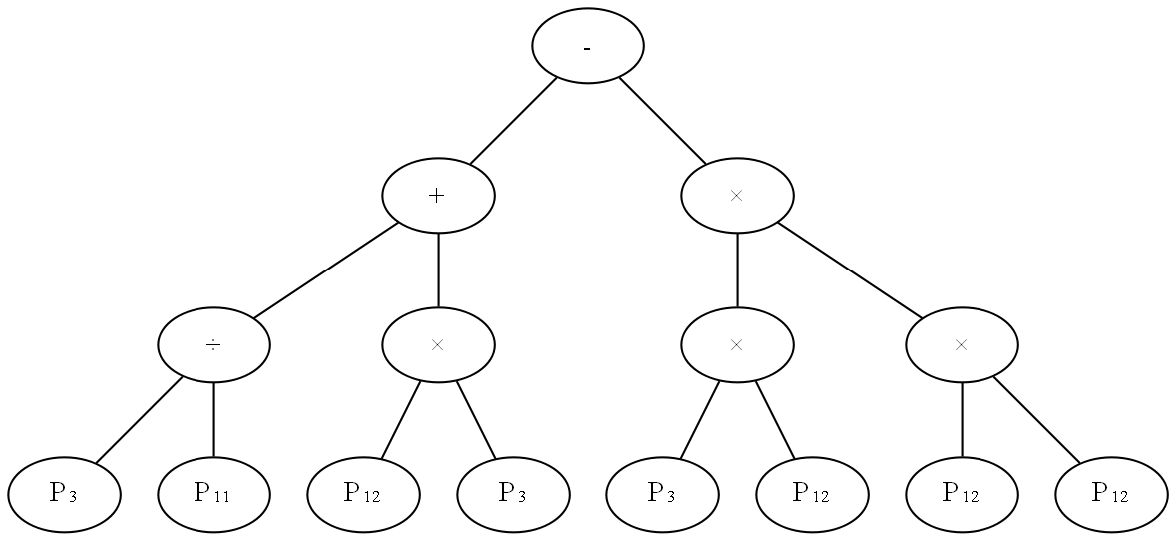
\includegraphics[width=1.0\textwidth]{figures/4-layer-gp.png}
    \caption{Four Layer GP Structure for Aseismic Programming} 
    \label{fig:4LGP}
  \end{center}
\end{figure}

%The performance of this model is not ideal because the RMSE can only reach 0.056. Based on Figure 9, the relationship model generated did not correctly build the relationship between the design parameters of school buildings, and ground acceleration of the minimum destruction. As only three input parameters were used, it resulted in the minimum equation as the linear equation. This can be attributed to the fact that this seismic ability model for school buildings has high complexity, and the application of GP pattern alone cannot obtain the relationship between them. The WGP pattern was then used to build the relationship equation between the design parameters of school buildings, and ground acceleration of the minimum destruction because it could be used for relationships that are more complex than with the GP pattern.

\begin{equation} AC = \dfrac{P_3}{P_{11}} + P_3 P_{12} - P_3 {P_{12}}^3  \label{eq:GP_AC}\end{equation}

\subsubsection{Weighted Genetic Programming}

WGP~是本分析第二個使用的方法,和~GP~一樣選擇了五層的運算樹,其他的基因演算的參數也都和~GP~分析中使用的一樣,~200~組基因演化~5000~代,交配率是~0.8~,突變率是~0.1~,而唯一不一樣的參數則是權重~$w$~的範圍,設定為~+10~到~-10~間,在此設定下分析~30~次,從中挑出表現最好的一組關係模型,其~RMSE~直在表二中,圖~\ref{fig:4LWGP}~是此關係模型的運算樹結構,其符號定義與~GP~方法運算樹使用的一樣,唯一不同的是黑色實心點,代表的是~$f = w_1x_1$~,此關係模型的方程式如下:

\begin{figure}[hbtp]
  \begin{center}
    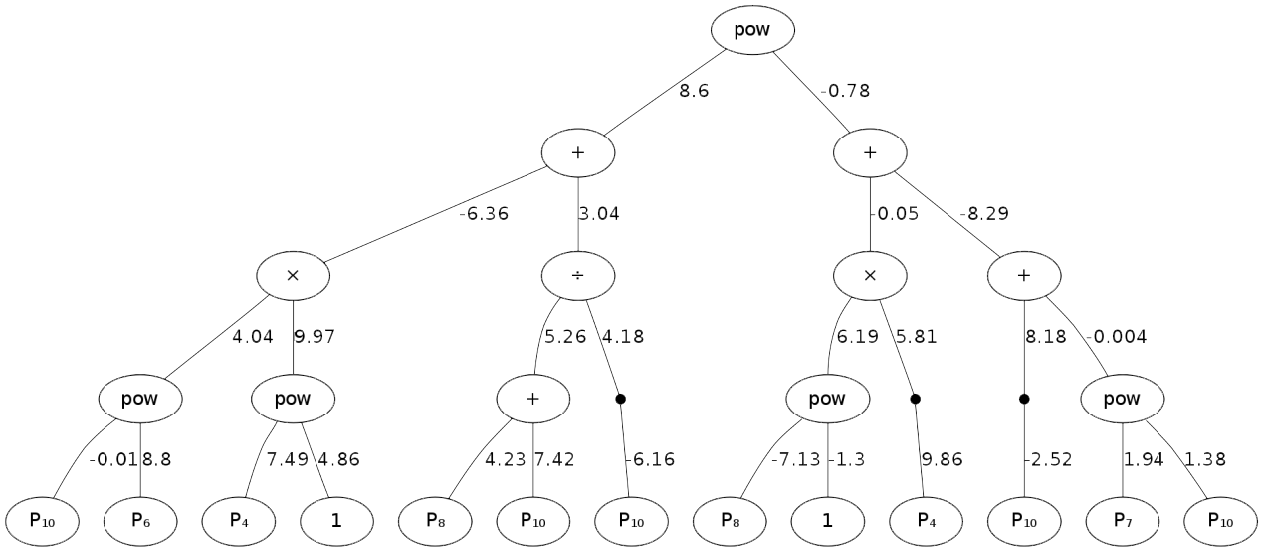
\includegraphics[width=1.0\textwidth]{figures/4-layer-wgp.png}
    \caption{Four Layer WGP Structure for Aseismic Programming} 
    \label{fig:4LWGP}
  \end{center}
\end{figure}


% WGP was used as the second model, which also chose five tiers of the operation tree. The optimum setting of GA is the same with GP: 200 populations of 5000 progressive iterations, a crossover rate of 0.8, and a mutation rate of 0.1. The best group was chosen after the analysis was conducted 30 times. Contrary to GP, the weight was set from +10 to -10 within the weighted (w) range. Table 2 shows the RMSE of the model generated, and the four-tier optimum equation is shown as Equation (9). The tree topology generated is displayed in Figure 10, and uses the same symbol as the GP tree topology to represent the same operator. The other symbol that was used is a black solid dot, which represents f=w1x1.

\begin{equation} AC = {({165 P_{10}}^{8.86 P_6} {P_4}^{4.86} + \dfrac{22.5 P_8 + 39.5 P_{10}}{P_{10}} )}^{-98.6 P_4{P_8}^{-1.3} - 133 P_{10} - 0.05 {P_7}^{1.38 P_{10}} }  \label{eq:WGP_AC}\end{equation}

表二列出了~WGP~方法所建立的校舍設計參數與其最所破壞地表加速度~$AC$~間關係模型的~RMSE~值,其值為~0.039~,比使用類神經網路所建立的關係模型表現還要好,圖~\ref{fig:WGP}~是此模型的推估值與實際直的比較圖,可以看得出來比使用~GP~所建立的模型要來的好。

\begin{figure}[hbtp]
  \begin{center}
    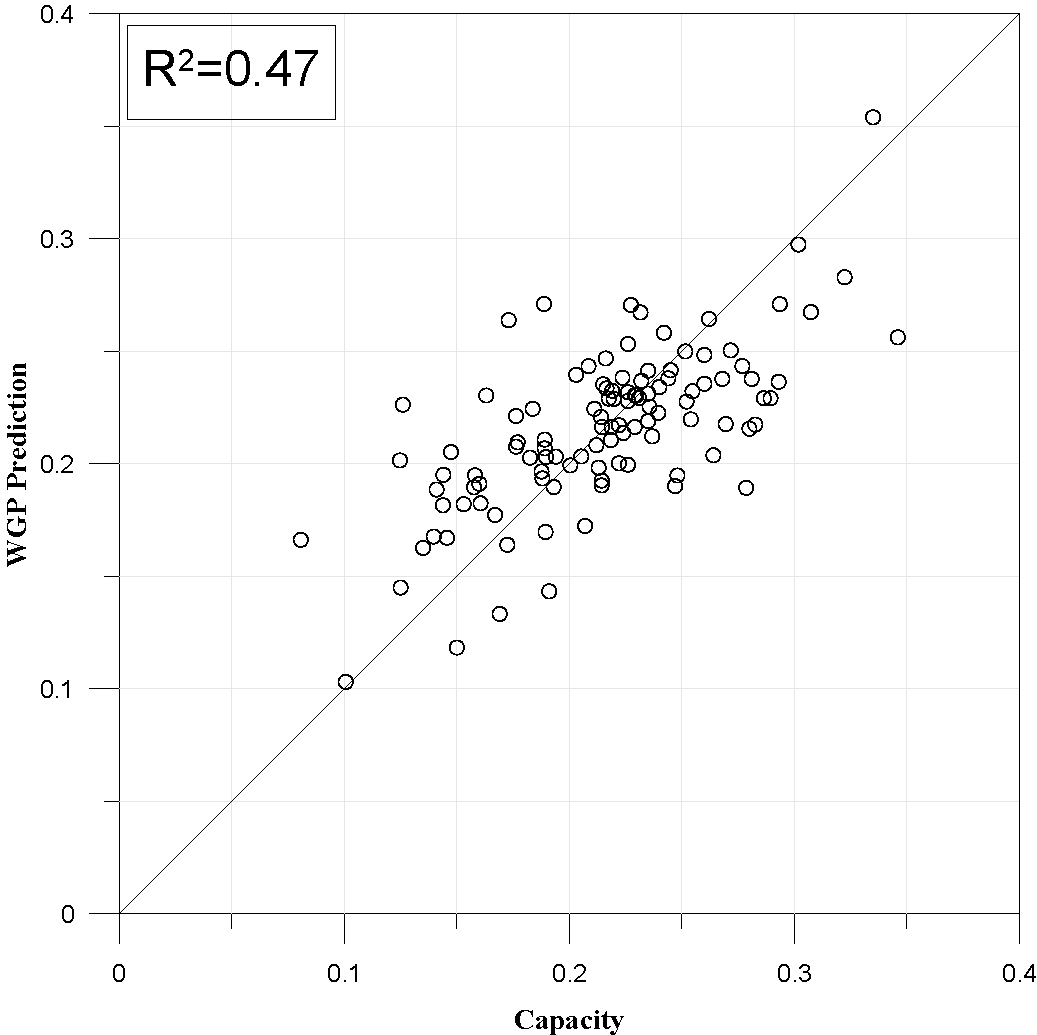
\includegraphics[width=0.75\textwidth]{figures/wgp.pdf}
    \caption{WGP Programming Result} 
    \label{fig:WGP}
  \end{center}
\end{figure}

% Table 2 shows the RMSE of the optimum relationship equations generated from the two patterns. The RMSE reached 0.039, which is better than the performance of the model built by the artificial neural networks in the contrast group. Figure 12 displays the comparison between the estimated, and the actual values of the model. By comparing the results, the model constructed by the WGP pattern is superior to the model constructed by the GP pattern.

本研究還分析了此關係模型所使用到的輸入參數,表三列出了此關係模型所有使用到的輸入參數,~$S_{DS}$~和~$S_{D1}$~並沒有被使用到,因其兩者都是和耐震需求相關的參數,而本分析的主要目標是校舍的地震承受能力,也就是耐震能力相關的部份,而此結果也正可以符合預期,而其餘所有的參數都有被使用到,也可以代表前處理所選擇到的參數都有其重要性。

% The parameters entered are analyzed based on the equation obtained from WGP, and Table 3 shows the input parameters obtained from the optimum relationship equations. SDS and SD1 were not used, as both are relevant to the demand of the CDR. For this study, the target is to estimate the Capacity (Aseismic Ability Index), which is irrelevant to Demand. Hence, this result conforms to the expectations. As all of the remaining input parameters were used, this indicates that the parameters chosen at the data processing stage are important.

\subsubsection{Capacity Index Formulation Tuning}

CDR~是詳細評估所得到的,校舍建築物的耐震能力指標,是校舍結構所能承受的地震力和規範所規定,校舍所在位置所需要能承受的地震力的比值,~CDR~大於~1~表示其耐震能力足夠,如果~CDR~等於~1~則表示耐震能力與需求相等,然而~$Is$~值的數量級和~CDR~不一樣,~$Is$~是百分系統,~100~表示耐震能力與需求相等,不過~$Is$~內其實還有一個調整參數~$I$~為~1.25~,而此時如果~$CDR$~是~1~則~$Is$~是~80~,這個關係可以用來將~$Is$~值轉為~$C_E$~值,其物理意義和~$AC$~相同。

% Similar with the CDR obtained from the detailed estimation, the aseismic capacity index of school buildings is the demand ratio of the aseismic capacity, excluding the ability unit and measure. CDR is directly compared to the ground acceleration, and IS is the estimated force ratio. If CDR is greater than 1, then the building has sufficient aseismic capacity. If CDR is 1, the building has an aseismic capacity equal to the demand. However, it should be noted that IS is a hundred-mark system, and 100 indicates that the capacity is equal to the demand. IS also needs to consider the usage coefficient I, of buildings. When IS equals 1.25, CDR is 1 and IS is 80. This relationship can be described by a formula that converts IS into CE, which has the same meaning as the ground acceleration of the minimum destruction.

\begin{equation} C_E = f(Is) = \dfrac{Is \times Demand \times I}{80}  \label{eq:CE}\end{equation}

$I$~是確保~$C_E$~值能趨於保守用的係數,在~NCREE~的設計中,校舍的~$I$~定為常數,為~1.25~,~$C_E$~即為最小破壞地表加速度,不過其可靠度較詳細評估所得到的數值低,因此本研究下一個分析目標即為修正初步評估的公式,為~$C_E$~加上一個調整因子~$T$~,可以讓其結果更接近詳細評估所得到的最小破壞地表加速度。

% I is the usage coefficient that intends to keep the seismic design at the conservative side, and prevents miscalculations caused by the insufficient estimation of the earthquake destruction. For this study, I is set to a constant of 1.25 for school buildings. Demand is set to different recommended values based on the positions of the school buildings. It represents the minimum ground acceleration that the buildings can withstand in the area. The School Building Database contains the demand data that was determined by engineers, based on the actual situations. This study adds T to CE as a revised formula, such that it is closer to the minimum destruction ground acceleration AC, of school buildings obtained from nonlinear analysis.

\begin{equation} AC = C_E + T  \label{eq:AC}\end{equation}

基於之前的結果,本分析只使用~WGP~來分析,基因演算的參數也和之前一樣,~4~或~5~層的運算樹,~200~個初始基因,~5000~個演化週期,交配率為~0.8~,突變率為~0.1~,訓練出~30~組模型後,從中挑選出最好的模型,結果~$T$~的模型為一個~4~層的運算樹,如圖~\ref{fig:4LWGPTuning}。

\begin{figure}[hbtp]
  \begin{center}
    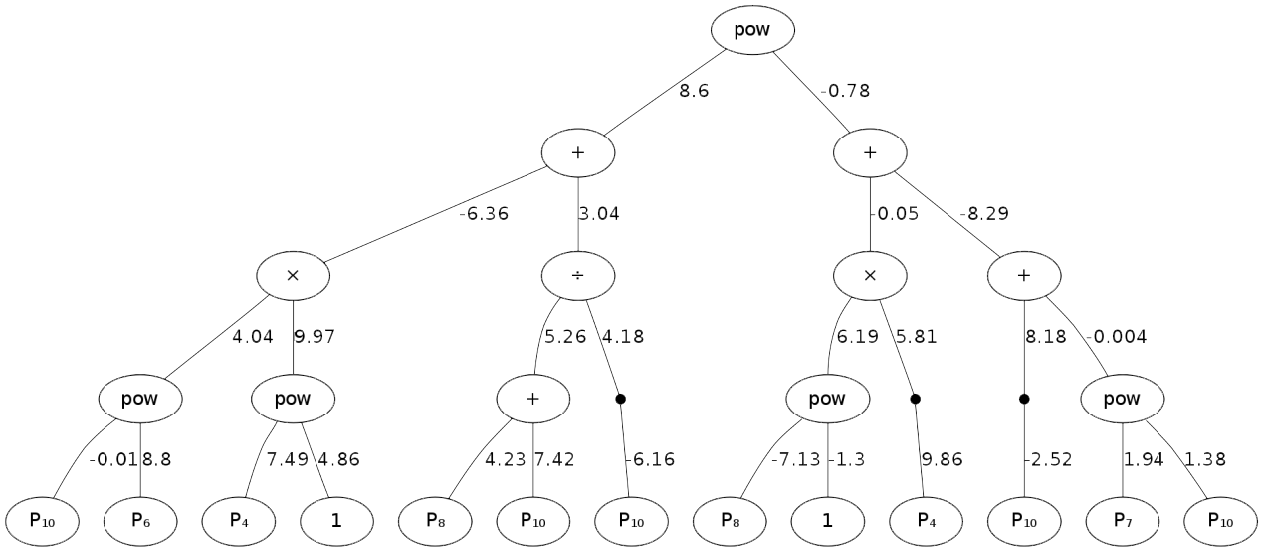
\includegraphics[width=1.0\textwidth]{figures/4-layer-wgp.png}
    \caption{Four Layer WGP Structure for Tuning Aseismic Ability Index} 
    \label{fig:4LWGPTuning}
  \end{center}
\end{figure}

% Based on the analysis above, this study only uses the WGP pattern to build the model, and this can be applied to complicated situations. Parameters chosen are: the operation tree has four to five tiers, 200 populations of 5000 progressive iterations, crossover rate of 0.8, mutation rate of 0.1, and choosing the best group after the analysis was conducted 30 times. The optimum T generated from the four-tier operation tree is shown in the equation below, and the tree topology is displayed in Figure 11.

\begin{equation} AC = C_E + 0.54 \dfrac{P_3}{P_2} - 24.86 \dfrac{ {P_6}^{0.36P_3} }{ {P_5}^{2.6P_9} } - ( 37.84 \dfrac{P_5}{0.67P_2 + 5.52P_7} )^{\left[ (-0.67 P_{12})^{1.23P_7/P_{13}} \right]} \label{eq:WGP_AC_IS}\end{equation}


\subsection{結果}

表二顯示了~NCREE~初步評估~$Is$~值轉換成詳細評估~$AC$~的等價數值~$C_E$~與校舍實際進行詳細評估所得到的最小破壞地表加速度~$AC$~相比的~RMSE~,為值~0.067~,距離目標的~0.04~還有一段距離,圖~\ref{fig:wgp-tuning}~是~$C_E$~與~$AC$~的比較圖,可以發現其趨勢相近,加上修正因子~$T$~之後,~RMSE~降低為~0.045~,圖~13~顯示了~$C_E + T$~和~$AC$~的比較,可以發現其趨勢更為接近,因此可以確定修正因子確實可以將初步評估的結果調整的更好。

\begin{figure}
  \begin{center}
    \subfigure[$C_E$]{
      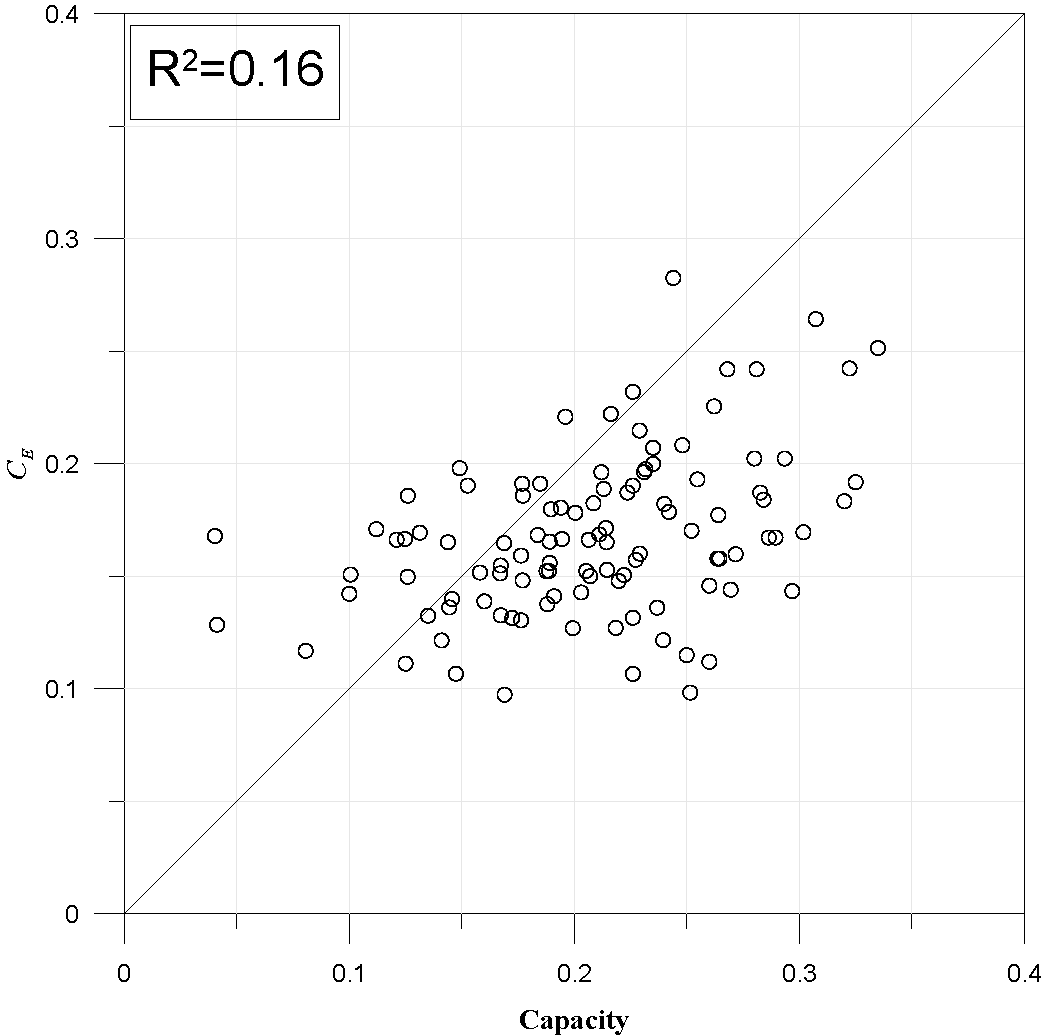
\includegraphics[width=0.65\textwidth]{figures/ce.pdf}
      \label{fig:ce}
    }
    \\
    \subfigure[$C_E+T$]{
      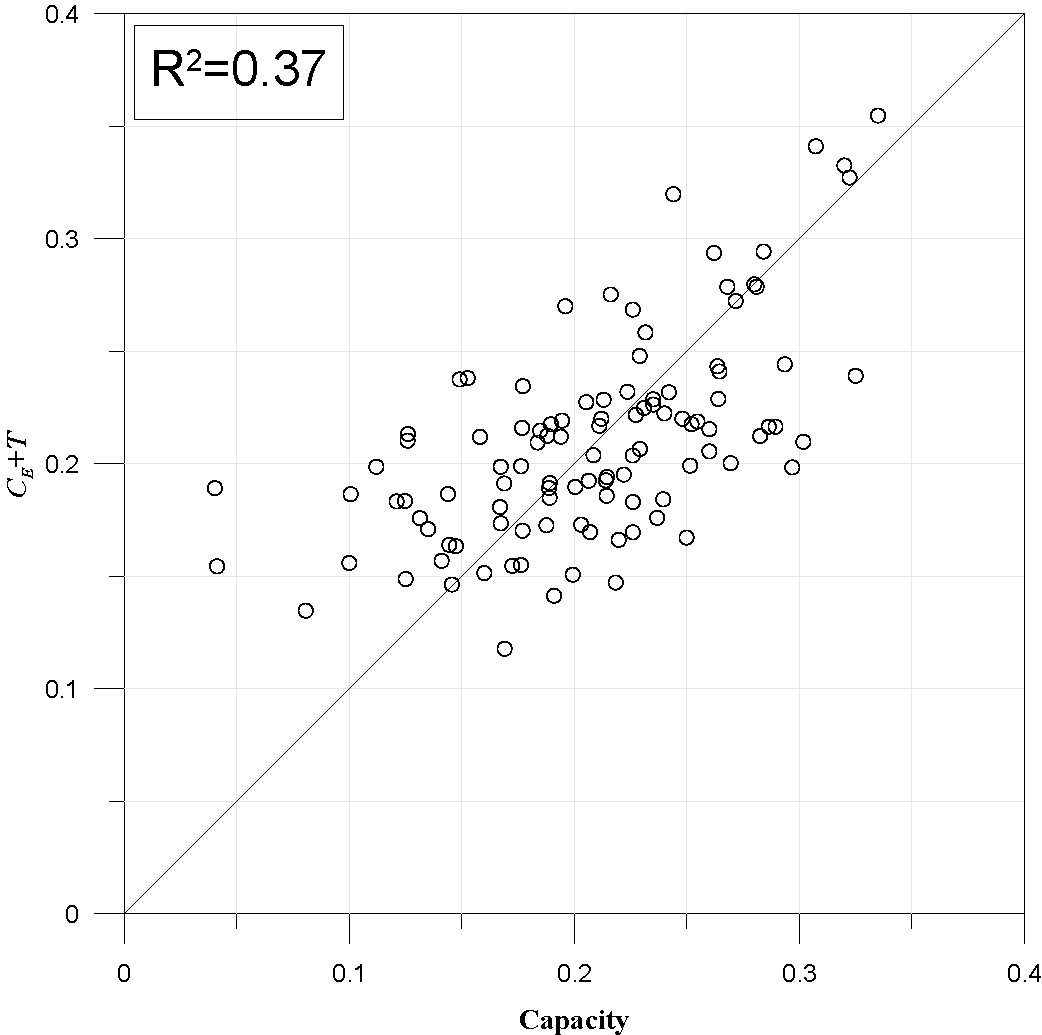
\includegraphics[width=0.65\textwidth]{figures/ce+T.pdf}
      \label{fig:cet}
    }
    \caption{WGP Tuning Result}
    \label{fig:wgp-tuning}
  \end{center}
\end{figure}

% Table 2 shows the RMSE after the revision. The RMSE of the IS formula used by NCREE in the preliminary appraisal is 0.067. Although there is still a gap between the target of 0.04 and this value, the emphasis is on the degree of relationship between them, and the main target is to screen out the school buildings with degrees of higher risk. Figure 13 shows the comparison between the CE converted from IS of NCREE, and the destructive ground acceleration obtained through linear analysis. Even though the data have the correct directional tendency, the model obtained from the GP method is better because of higher deviation, and a linear relationship. Subsequent to adding T to the revised formula, RMSE is reduced to 0.045. Figure 13 shows the comparison, and it can be seen that the directional tendency is quite close, thus reducing the deviation. A good revision effect is observed, making the screening result of the preliminary appraisal more accurate.

表三呈現了此分析中所有使用到的輸入參數,四層運算樹和五層運算數分別使用到的參數分開表示,其中:樓層數($P_1$)、總樓地板面積($P_{10}$)和單間教室的垮數($P_{13}$)並沒有被使用到,其中前兩個參數對於校舍結構的耐震能力來說非常重要,在~$Is$~的推估過程中已經有使用到,而本分析的修正因子並沒有使用到可以顯示~NCREE~的初步評估已經很完整正確的表現出這兩個參數所造成的影響,而單間教室垮數的資訊則可能在初步評估的過程中已經將該資訊表現在評估公式內了,因此修正因子~$T$~的公式內並不包含它,不過此參數在前一個分析中依然有使用到,因此仍然有其重要性。

% Table 3 shows the input parameters used by the equation obtained from the WGP method, and by the optimum relationship equations with four to five tiers. The number of floors (P1), total floorage (P10), and number of spans in a single classroom (P13) were not used because the number of floors and total floorage, which are highly important, were already used in the IS formula. Hence, IS has been correctly included in the two properties above, and the number of spans in a single classroom can be inferred as hidden in the formula. Hence, T in the revised formula will not use this input parameter. However, the input parameter is still used to directly construct the relationship equation in the previous case, and has a certain degree of importance.



% In order to estimate the aseismic ability of a building, we need to obtained detailed information about its geometric dimensions, the properties of materials used, etc. and we may need to perform sampling and other experiments to obtain certain information e.g. the properties of materials used. Based on this information, a structural model of the building has to be constructed and then non-linear pushover analysis is used to perform estimation. This process is time-consuming, and technicians are required. It usually takes about one months to estimate the aseismic ability of a building.

在校舍資訊與耐震能力之關係模型之分析中,本研究提出了基於~WGP~方法所建立的關係模型,只要透過校舍結構的基本參數就可以推估校舍的耐震能力,其前處理的工作可以分為兩個部分,第一個部分是資料的過濾與挑選,其而過濾與挑選的條件是基於專家的建議,第二個部分是找出不同資料屬性的重要性,第一步是先將和校舍結構非關以及明確不重要的資料屬性剃除,接著藉由將校舍分成不同子集,並逐步減少資料屬性,最後選出了~14~個資料屬性,然後基於這個子集進行資料探勘分析,相較於原來上百個資料屬性,本分析達到了一個非常高效的資料壓縮,減少了非常多的資料雜訊。

% In this study, we adopted the WGP method to construct a relation model, which uses the basic design parameters of school buildings to estimate their aseismic ability. The pre-processing efforts carried out for the proposed prediction model can be divided into two parts. The first part is a data filter for selecting out data sets which are reasonable as typical school buildings. The selection conditions of this data filter is proposed based on judgment with expertise in structural engineering. The second part is the determination of the key properties used in the proposed model. We first eliminate some properties which are non-structural and low importance, and synthesize some properties with similarity. We further classifies school building records into subsets based on similarities in property values, and chooses one subset with major population as the data set for further studying. Based on this subset, we try to do further reduction and finally determine 14 properties which are optimal to represent the seismic characteristics of individual school buildings. In comparison with hundreds of properties in the original data, a very high reduction ratio is reached.

WGP~最大的特色就是其產生的模型結果是使用數學方程式的形式來呈現,因此可以很簡單的就將產出的模型拿到不同的系統或平台中應用,除~WGP~外,本分析也使用了~GP~來進行分析,經過比較可以發現~WGP~方法所建立的模型的表現要比~GP~方法的好很多,可以顯示其對於複雜問題的處理能力是更為優秀的,而其~RMSE~也可以低於~0.04~,比類神經網路的表現還優秀,透過預測值與實際直的比較圖,也可以發現其趨勢都是正相關,驗證了使用挑選出的~14~個參數和~WGP~方法所建立的關係模型是可以在校舍補強工作上使用的。

% Same as GP, a key characteristic of WGP is the resulting model is in the form of mathematic equation, which is very easy and convenient to be applied in engineering practice, and thus is more practical than other soft computing methods. This study also applies GP on the same set of school building data for predicting the building’s collapse ground acceleration. Compared to the prediction results by using GP, the accuracy of WGP model is much better. This case shows WGP can handle problems with more complexities than GP. Regarding the application of WGP method, this study performs 5000 iterations of revolutions for test models with operation tree from two to five levels respectively, and determines the optimized values of model parameters, such as the crossover rate and mutation rate, for this application case through repeated tests. The RMSE of the resulting model achieves less than 0.04. This accuracy in prediction is comparable with the model using Artificial Neural Networks (ANNs). In addition, the graph compared the actual values with predict values shows the distribution trend of the data points are consistent with the expected direction. The result verification indicates the proposed WGP-based model successfully establishes the relation between the 14 input properties and the output property, building’s collapse ground acceleration. In practice, the proposed model can be applied directly and efficiently for preliminary assessment of school buildings for seismic capacities.



% In addition to directly inferring the aseismic capacity of school buildings from the design parameters, the current study revised the aseismic capacity index formula of school buildings designed by NCREE using GPS. The formula was to provide greater accuracy with a smaller deviation. This model can help decision makers with issues that are related to the aseismic capacity of school buildings, as well as estimating the disaster loss, during a disaster in a timely manner. These applications require that the estimation of the aseismic capacity of many school buildings be generated rapidly, and this would be impossible if traditional non-linear structural analysis were applied.


